\documentclass{dlproblemset}
\usepackage{tikz}
\tikzset{every picture/.style={line width=0.75pt}}

% Cores e estilos da célula recorrente (mesma convenção dos slides)
\definecolor{PastelBlue}{HTML}{BCD8EC}
\definecolor{PastelPink}{HTML}{FFCBE1}
\definecolor{PastelGreen}{HTML}{D6E5BD}
\definecolor{PastelYellow}{HTML}{F9E1A8}
\tikzset{
    rnncell/.style={draw, rounded corners, fill=PastelGreen, minimum width=1.6cm, minimum height=1.0cm},
    inputnode/.style={circle, draw, fill=PastelBlue, minimum size=0.7cm, inner sep=1pt, font=\small},
    outputnode/.style={circle, draw, fill=PastelPink, minimum size=0.7cm, inner sep=1pt, font=\small},
    opnode/.style={draw, fill=PastelYellow, rounded corners=2pt, font=\scriptsize, inner sep=2pt}
}

\title{Redes Recorrentes}
\subtitle{Lista de Exercícios}

\begin{document}

\begin{enumerate}[I)]

\subsection*{Redes Recorrentes}
    \item Qual é a principal vantagem das redes neurais recorrentes (RNNs) em relação a MLPs e redes convolucionais?

    \item  Descreva a estrutura de uma RNN básica.

    \item Em frameworks de desenvolvimento de redes neurais (como o PyTorch) é comum que o bloco de rede recorrente conte apenas com a camada densa que computa o estado oculto (\textit{hidden state}) e que não conte com a camada densa que computa a saída. Qual motivo disso? 

    \item Uma rede recorrente tem um limite teórico para o tamanho de sequências que consegue processar? E do ponto de vista prático, existem limites?

    \item Redes recorrentes tendem a sofrer mais dos problemas do gradiente que se dissipa e do gradiente explosivo. Por que isso acontece?

    \item \textit{(Adaptado de CS224N Stanford 2017)} Considere que todos os parâmetros da rede recorrente ilustrada na figura abaixo são escalares ($\theta_{hh}, \theta_{ih}, b_{h}, \theta_{ho}$ e  $b_{o}$). A função de ativação $f[.]$ é a função sinal definida abaixo:
    
\[   
f(z) = 
     \begin{cases}
       z \ge 0, &\quad 1,\\
       z < 0, &\quad 0\\
     \end{cases}
\]
    
    Sua tarefa é descobrir valores para esses parâmetros que façam a rede recorrente ter como saída inicial o valor $0$ e, assim que ela receba um valor $1$ como entrada ela passe a ter como saída o valor $1$ para toda e qualquer entrada futura.
    Por exemplo: Se a entrada for 00110 a saída deve ser 00111.
    \begin{figure}[H]
        \centering
        \resizebox{0.5\linewidth}{!}{%
        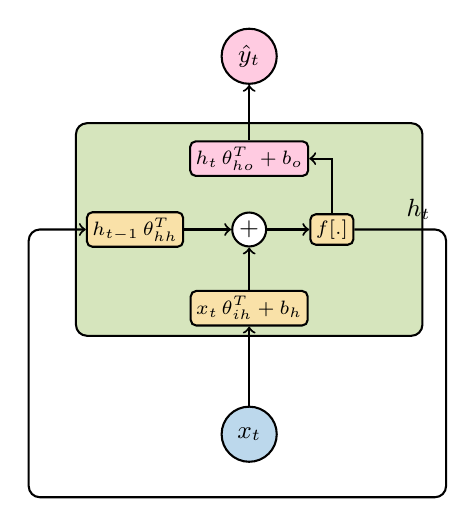
\begin{tikzpicture}[every node/.style={font=\small}]
            \node[rnncell, minimum width=4.4cm, minimum height=2.7cm] (cell) at (0.1, 0.4) {};
            \node[opnode] (hh) at (-1.35, 0.4) {$h_{t-1}\,\theta_{hh}^{T}$};
            \node[draw, circle, inner sep=1pt, fill=white] (plus) at (0.1, 0.4) {$+$};
            \node[opnode] (act) at (1.15, 0.4) {$f[.]$};
            \node[opnode] (xh) at (0.1, -0.6) {$x_t\,\theta_{ih}^{T} + b_h$};
            \node[opnode, fill=PastelPink] (out) at (0.1, 1.3) {$h_t\,\theta_{ho}^{T} + b_o$};
            \node[inputnode] (xnode) at (0.1, -2.2) {$x_t$};
            \node[outputnode] (ynode) at (0.1, 2.6) {$\hat{y}_t$};
            \draw[->] (xnode) -- (xh);
            \draw[->] (xh) -- (plus);
            \draw[->] (hh) -- (plus);
            \draw[->] (plus) -- (act);
            \draw[->] (act) |- (out);
            \draw[->] (out) -- (ynode);
            % estado interno h_t: sai e retorna (recorrência)
            \draw[->, rounded corners=4pt] (act.east) -- (2.6, 0.4) node[above, pos=0.7] {$h_t$}
                -- (2.6, -3.0) -- (-2.7, -3.0) -- (-2.7, 0.4) -- (hh.west);
        \end{tikzpicture}}
        \caption{RNN para questão VI}
        \label{fig:rnn}
    \end{figure}

    \item 
        Considere uma rede híbrida que faz \textit{Image Captioning} (gera legendas para imagens). A arquitetura é composta por um \textit{encoder} (uma CNN pré-treinada, como a VGG-16) e um \textit{decoder} (uma RNN simples). O encoder recebe como input uma imagem $I$ e sua saída serve de entrada para o decoder, que então é responsável pela geração de legenda, uma palavra de cada vez ($y_1, y_2, ..., y_n$...).
        Com base neste cenário, responda:
    
        \begin{enumerate}[a)]
            \item Caso utilizemos uma VGG-16, qual é o papel dela nesta tarefa? E qual é o papel da RNN? Por que não podemos usar apenas a VGG-16 para a tarefa inteira?
            
            % \item Descreva conceitualmente como a informação é "entregue" da CNN para a RNN.
            
            \item Este processo de geração de palavras é autorregressivo. Descreva o que serve como input ($x_t$) e o que serve como estado oculto anterior ($h_{t-1}$) para a RNN nos seguintes passos de tempo:
                \begin{enumerate}[i.)]
                    \item Para gerar a primeira palavra ($y_1$) no tempo $t=1$.
                    \item Para gerar a segunda palavra ($y_2$) no tempo $t=2$.
                \end{enumerate}
            
            \item A CNN (Encoder) processa a imagem uma única vez para gerar um vetor de contexto $v$. Qual é a origem e o formato (shape) mais comum deste vetor $v$? Ele é a saída da última camada convolucional (um tensor 3D), ou é a saída que foi "achatada" (flattened), ou é a saída já processada de uma camada totalmente conectada (FC)?

            \item Digamos que não queremos perder a informação espacial de cada frame ao passá-la para a RNN. Ou seja, queremos que o \textit{input} $x_t$ e o \textit{estado oculto} $h_t$ sejam eles mesmos mapas de características 3D (ex: [Altura, Largura, Canais]), e não vetores 1D. É possível utilizar operações de convolução \emph{dentro} da célula da RNN (para calcular $h_t$ a partir de $h_{t-1}$ e $x_t$) em vez das multiplicações de matrizes (camadas densas) tradicionais? Explique brevemente o conceito.
        \end{enumerate}

    \item Considere uma vanilla RNN escalar com pesos $\theta_{hh} = 0.3$, $\theta_{ih} = 0.8$, $\theta_{ho} = 1.0$, \textit{bias} $b_h = b_o = 0$, ativação $\tanh$ e estado inicial $h_0 = 0$. A célula é definida por
    \[
        h_t = \tanh(x_t\,\theta_{ih} + h_{t-1}\,\theta_{hh}), \qquad \hat{y}_t = h_t\,\theta_{ho}.
    \]
    A rede recebe a sequência $x = [1.0,\, -0.5]$ e deve prever, ao final do segundo passo, o alvo $y = 1.0$. A \textit{loss} é o MSE, $J = \tfrac{1}{2}(\hat{y}_2 - y)^2$.
    \begin{enumerate}[a)]
        \item Compute o \textit{forward pass}: $z_1$, $h_1$, $z_2$, $h_2$, $\hat{y}_2$ e $J$.
        \item Compute $\partial J / \partial \theta_{ho}$.
        \item Compute $\partial J / \partial \theta_{hh}$ via \textit{backpropagation through time}, mostrando os gradientes intermediários $\partial J / \partial h_2$, $\partial J / \partial z_2$, $\partial J / \partial h_1$ e $\partial J / \partial z_1$.
    \end{enumerate}

    \item \textbf{Perplexidade}: um \textit{language model} atribui, a uma sequência de $m = 4$ \textit{tokens}, as probabilidades condicionais
    \[
        p(y_t \mid y_{<t}) = [\,0.25,\; 0.5,\; 0.125,\; 0.5\,].
    \]
    Calcule a perplexidade do modelo nessa sequência (usando a definição $\text{Perplexidade} = 2^{-L/m}$ com $L = \sum_t \log_2 p(y_t \mid y_{<t})$) e interprete o resultado em termos do ``número médio efetivo de \textit{tokens}'' entre os quais o modelo está em dúvida.

\end{enumerate}

\newpage
\subsection*{Gabarito}
\color{blue}

\begin{enumerate}[I)]

    \item As RNNs podem capturar e analisar informações sequenciais, tornando-as adequadas para tarefas que envolvem séries temporais, processamento de linguagem natural e dados sequenciais. Elas atingem esse feito usando uma recorrência, ou seja, um estado oculto da rede é computado e serve como entrada para o processamento do próximo item da sequência.


    \item Uma RNN consiste em uma camada de entrada, uma camada oculta com conexões recorrentes e uma camada de saída. A camada oculta mantém um estado oculto que é atualizado a cada passo temporal, e é usado como entrada para os passos subsequentes, permitindo que a rede memorize informações de entradas anteriores.

    \item As tarefas que envolvem dados sequenciais são muito variadas. Podemos fazer análise de sentimentos (classificar uma sequência), \textit{image captioning} no qual temos uma entrada e uma sequência como saída ou ainda sequence-to-sequence onde temos sequências na entrada e na saída. Dada essa grande variedade de problemas, seria um desperdício manter parâmetros de saída para cada unidade recorrente. Mantendo a unidade recorrente sem saída por padrão, os \textit{frameworks} transferem a responsabilidade de definir quando a saída deve ser computada (e onde os parâmetros devem ser aprendidos) para o desenvolvedor.

    \item Do ponto de vista teórico uma RNN consegue processar entradas de qualquer tamanho, um item por vez. Contudo, na prática vemos que RNN não trabalham bem com dependências muito longas. Isso ocorre pois em RNN estamos sempre atualizando o estado oculto em cada uma das iterações ao longo do tempo.

    \item Redes recorrentes são mais sensíveis a esse tipo de problema pois além de serem profundas no número de camadas elas são profundas também na dimensão tempo. Dessa forma, durante o \textit{backpropagation through time} o gradiente sofre mais multiplicações e é acumulado em múltiplas iterações potencializando ambos problemas.

    \item Existem muitas soluções para essa questão. A solução abaixo é apenas uma das possibilidades:
    
    $\theta_{hh}=1$

    $\theta_{ih}=1$

    $b_{h}= -1$

    $\theta_{ho}=1$

    $b_{o}=0$
    
    \item 
        \begin{enumerate}[a)]
            \item Sua função é processar a imagem, analisando e extraindo as características visuais importantes, comprimindo toda a informação em um único vetor ($v$). Usando uma VGG-16 de encoder (como a VGG) não é possível, sozinha, gerar uma saída sequencial. A tarefa de decoder sequencial (gerar uma frase) requer uma arquitetura diferente, como uma RNN ou um Transformer.

            % \item Sua função é processar dados sequenciais, recebendo o vetor $v$ e utilizando ele como ponto de partida para gerar uma sequência de palavras gramaticalmente correta que descreva o contexto visual. Tecnicamente é possível alimentar uma RNN com pixels em sequência, porém ela é inadequada para entender a estrutura espacial 2D de uma imagem e falha em capturar relações de longo alcance, sendo uma escolha ineficiente como encoder de imagens.

            \item O processo é chamado de autorregressivo porque a saída de um passo de tempo é usada como entrada para o próximo passo.
                        \begin{enumerate}[i.]
                            \item \textbf{Para gerar $y_1$ (Tempo $t=1$):}
                                \begin{itemize}
                                    \item \textbf{Estado Oculto Anterior ($h_{t-1}$):} É o $h_0$, que é o vetor da imagem $v$ fornecido pela CNN.
                                    
                                    \item \textbf{Input ($x_1$):} Não temos uma palavra anterior. Portanto, usamos um \textit{token} especial de início de sentença (ex: \texttt{<START>}).
                                    
                                    \item \textbf{Cálculo:} $h_1 = f(x_1\,\theta_{ih}^{T} + v\,\theta_{hh}^{T} + b_h)$ e $y_1 = g(h_1\,\theta_{ho}^{T} + b_o)$.
                                \end{itemize}
                        
                            \item \textbf{Para gerar $y_2$ (Tempo $t=2$):}
                                \begin{itemize}
                                    \item \textbf{Estado Oculto Anterior ($h_{t-1}$):} É o $h_1$, o estado oculto que acabou de ser calculado no passo anterior.
                                    
                                    \item \textbf{Input ($x_2$):} É a palavra que foi gerada no passo anterior, ou seja, $y_1$.
                                    
                                    \item \textbf{Cálculo} $h_2 = f(y_1\,\theta_{ih}^{T} + h_1\,\theta_{hh}^{T} + b_h)$ e $y_2 = g(h_2\,\theta_{ho}^{T} + b_o)$.
                                \end{itemize}
                        \end{enumerate}

            \item A abordagem mais comum e direta \textbf{é} usar a saída `achatada' (flattened) da última camada convolucional.
                \begin{enumerate}[i.]
                    \item Processo: A imagem passa pelas camadas convolucionais (ex: VGG-16), resultando em um \textit{feature map} 3D (ex: $7 \times 7 \times 512$). Achatamos (flattening) para um vetor 1D (ex: $25088 \times 1$). A saída é usada como o vetor $v$.
                    \item Formato (Shape): O vetor $v$ é um vetor 1D (ex: `($25088$,)').
                    \item Uso: Este vetor 1D representa a imagem inteira, é usado para inicializar o primeiro estado oculto ($h_0$) da RNN, `preparando' o decoder com o que ele deve descrever.
                \end{enumerate}

            \item Sim, é possível, e esta arquitetura é conhecida como \textbf{Convolutional RNN} (ou ConvLSTM/ConvGRU).
                \begin{enumerate}[i.]
                    \item Conceito: Em uma RNN padrão, o cálculo do novo estado oculto envolve multiplicações de matrizes (camadas densas):
                    $$
                    h_t = \tanh(x_t\,\theta_{ih}^{T} + h_{t-1}\,\theta_{hh}^{T} + b_h)
                    $$
                    Exigindo que $h_t$, $h_{t-1}$ e $x_t$ sejam vetores 1D.

                    \item Em uma ConvRNN: As multiplicações de matrizes por $\theta_{ih}$ e $\theta_{hh}$ são substituídas por operações de convolução. Neste caso, o \textit{input} $x_t$ é o próprio mapa de características 3D da CNN (ex: $7 \times 7 \times 512$). É necessário que sejam preservadas as dimensões espaciais, permitindo que a RNN "lembre" não apenas o que viu nos frames anteriores, mas onde (espacialmente) viu.
                \end{enumerate}

        \end{enumerate}

    \item \textit{Forward} e BPTT na vanilla RNN escalar.
    \begin{enumerate}[a)]
        \item \textit{Forward pass}:
        \begin{align*}
            z_1 &= x_1\,\theta_{ih} + h_0\,\theta_{hh} = 1.0\cdot 0.8 + 0\cdot 0.3 = 0.8 \\
            h_1 &= \tanh(0.8) \approx 0.6640 \\
            z_2 &= x_2\,\theta_{ih} + h_1\,\theta_{hh} = (-0.5)\cdot 0.8 + 0.6640\cdot 0.3 \approx -0.2008 \\
            h_2 &= \tanh(-0.2008) \approx -0.1982 \\
            \hat{y}_2 &= h_2\,\theta_{ho} \approx -0.1982 \\
            J &= \tfrac{1}{2}(\hat{y}_2 - y)^2 \approx \tfrac{1}{2}(-1.1982)^2 \approx 0.7178
        \end{align*}

        \item Derivada em $\theta_{ho}$:
        \[
            \frac{\partial J}{\partial \theta_{ho}} = (\hat{y}_2 - y)\,h_2 \approx -1.1982 \cdot (-0.1982) \approx 0.2374.
        \]

        \item BPTT para $\theta_{hh}$. Gradientes intermediários:
        \begin{align*}
            \frac{\partial J}{\partial h_2} &= (\hat{y}_2 - y)\,\theta_{ho} \approx -1.1982 \\
            \frac{\partial J}{\partial z_2} &= \frac{\partial J}{\partial h_2}\,(1 - h_2^2) \approx -1.1982 \cdot (1 - 0.0393) \approx -1.1511 \\
            \frac{\partial J}{\partial h_1} &= \frac{\partial J}{\partial z_2}\,\theta_{hh} \approx -1.1511 \cdot 0.3 \approx -0.3453 \\
            \frac{\partial J}{\partial z_1} &= \frac{\partial J}{\partial h_1}\,(1 - h_1^2) \approx -0.3453 \cdot (1 - 0.4410) \approx -0.1931
        \end{align*}
        A contribuição direta de $\theta_{hh}$ em $t=2$ tem fator $h_1$; em $t=1$ tem fator $h_0 = 0$, anulando o termo. Logo,
        \[
            \frac{\partial J}{\partial \theta_{hh}} = \frac{\partial J}{\partial z_2}\,h_1 + \frac{\partial J}{\partial z_1}\,h_0 \approx -1.1511 \cdot 0.6640 + 0 \approx -0.7644.
        \]
    \end{enumerate}

    \item Perplexidade. Calculando $\log_2$ de cada probabilidade:
    \[
        \log_2 p = [-2,\; -1,\; -3,\; -1] \quad\Rightarrow\quad L = \sum_t \log_2 p_t = -7.
    \]
    Expoente da perplexidade: $-L/m = 7/4 = 1.75$. Portanto,
    \[
        \text{Perplexidade} = 2^{1.75} \approx 3.364.
    \]
    Interpretação: em média, o modelo se comporta, em cada passo, como se estivesse em dúvida entre cerca de $3.4$ \textit{tokens} igualmente prováveis.

\end{enumerate}

\end{document}
